\documentclass[14pt]{extbook}
\usepackage{multicol, enumerate, enumitem, hyperref, color, soul, setspace, parskip, fancyhdr} %General Packages
\usepackage{amssymb, amsthm, amsmath, bbm, latexsym, units, mathtools} %Math Packages
\everymath{\displaystyle} %All math in Display Style
% Packages with additional options
\usepackage[headsep=0.5cm,headheight=12pt, left=1 in,right= 1 in,top= 1 in,bottom= 1 in]{geometry}
\usepackage[usenames,dvipsnames]{xcolor}
\usepackage{dashrule}  % Package to use the command below to create lines between items
\newcommand{\litem}[1]{\item#1\hspace*{-1cm}\rule{\textwidth}{0.4pt}}
\pagestyle{fancy}
\lhead{Module12L}
\chead{}
\rhead{Version C}
\lfoot{9732-2394}
\cfoot{}
\rfoot{Fall 2020}
\begin{document}

\begin{enumerate}
\litem{
Determine the horizontal and/or oblique asymptotes in the rational function below.\[ f(x) = \frac{6x^{3} +11 x^{2} -x -6}{2x^{2} -3 x -9} \]\begin{enumerate}[label=\Alph*.]
\item \( \text{Oblique Asymptote of } y = 3x + 10. \)
\item \( \text{Horizontal Asymptote of } y = 3.0  \)
\item \( \text{Horizontal Asymptote at } y = 3.0 \)
\item \( \text{Horizontal Asymptote of } y = 3.0 \text{ and Oblique Asymptote of } y = 3x + 10 \)
\item \( \text{Horizontal Asymptote of } y = 3.0 \text{ and Oblique Asymptote of } y = 3x + 10 \)

\end{enumerate} }
\litem{
Determine the horizontal and/or oblique asymptotes in the rational function below.\[ f(x) = \frac{6x^{3} +7 x^{2} -50 x -75}{3x^{2} +20 x + 25} \]\begin{enumerate}[label=\Alph*.]
\item \( \text{Horizontal Asymptote of } y = -5.0 \text{ and Oblique Asymptote of } y = 2x -11 \)
\item \( \text{Horizontal Asymptote of } y = 2.0  \)
\item \( \text{Horizontal Asymptote of } y = 2.0 \text{ and Oblique Asymptote of } y = 2x -11 \)
\item \( \text{Horizontal Asymptote at } y = -5.0 \)
\item \( \text{Oblique Asymptote of } y = 2x -11. \)

\end{enumerate} }
\litem{
Which of the following functions \textit{could} be the graph below?
\begin{center}
    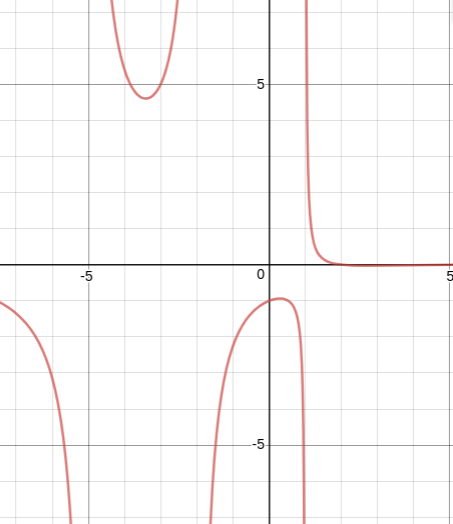
\includegraphics[width=0.5\textwidth]{../Figures/identifyGraphOfRationalFunctionC.png}
\end{center}
\begin{enumerate}[label=\Alph*.]
\item \( f(x)=\frac{x^{3} +18 x^{2} +107 x + 210}{x^{3} -7 x^{2} +4 x + 12} \)
\item \( f(x)=\frac{x^{3} +10 x^{2} +11 x -70}{x^{3} -7 x^{2} +4 x + 12} \)
\item \( f(x)=\frac{x^{3} -10 x^{2} +11 x + 70}{x^{3} +7 x^{2} +4 x -12} \)
\item \( f(x)=\frac{x^{3} -10 x^{2} +11 x + 70}{x^{3} +7 x^{2} +4 x -12} \)
\item \( \text{None of the above are possible equations for the graph.} \)

\end{enumerate} }
\litem{
Determine the vertical asymptotes and holes in the rational function below.\[ f(x) = \frac{6x^{3} +43 x^{2} +91 x + 60}{12x^{2} +5 x -25} \]\begin{enumerate}[label=\Alph*.]
\item \( \text{Vertical Asymptote of } x = 0.5 \text{ and hole at } x = -1.667 \)
\item \( \text{Holes at } x = 1.25 \text{ and } x = -1.667 \text{ with no vertical asymptotes.} \)
\item \( \text{Vertical Asymptotes of } x = 1.25 \text{ and } x = -1.5 \text{ with a hole at } x = -1.667 \)
\item \( \text{Vertical Asymptotes of } x = 1.25 \text{ and } x = -1.667 \text{ with no holes.} \)
\item \( \text{Vertical Asymptote of } x = 1.25 \text{ and hole at } x = -1.667 \)

\end{enumerate} }
\litem{
Determine the horizontal and/or oblique asymptotes in the rational function below.\[ f(x) = \frac{2x^{2} +x -15}{4x^{3} -20 x^{2} +x + 60} \]\begin{enumerate}[label=\Alph*.]
\item \( \text{Horizontal Asymptote of } y = 0 \)
\item \( \text{Oblique Asymptote of } y = 2x -11. \)
\item \( \text{Horizontal Asymptote of } y = 2.000 \text{ and Oblique Asymptote of } y = 2x -11 \)
\item \( \text{Horizontal Asymptote at } y = -3.000 \)
\item \( \text{Horizontal Asymptote of } y = 2.000  \)

\end{enumerate} }
\litem{
Determine the vertical asymptotes and holes in the rational function below.\[ f(x) = \frac{6x^{3} -19 x^{2} + 25}{9x^{2} -3 x -20} \]\begin{enumerate}[label=\Alph*.]
\item \( \text{Holes at } x = -1.333 \text{ and } x = 1.667 \text{ with no vertical asymptotes.} \)
\item \( \text{Vertical Asymptote of } x = 0.667 \text{ and hole at } x = 1.667 \)
\item \( \text{Vertical Asymptotes of } x = -1.333 \text{ and } x = 2.5 \text{ with a hole at } x = 1.667 \)
\item \( \text{Vertical Asymptotes of } x = -1.333 \text{ and } x = 1.667 \text{ with no holes.} \)
\item \( \text{Vertical Asymptote of } x = -1.333 \text{ and hole at } x = 1.667 \)

\end{enumerate} }
\litem{
Determine the horizontal and/or oblique asymptotes in the rational function below.\[ f(x) = \frac{2x^{2} -3 x -20}{8x^{3} +34 x^{2} +41 x + 15} \]\begin{enumerate}[label=\Alph*.]
\item \( \text{Horizontal Asymptote of } y = 4.000 \text{ and Oblique Asymptote of } y = 4x + 23 \)
\item \( \text{Horizontal Asymptote of } y = 4.000  \)
\item \( \text{Horizontal Asymptote of } y = 0 \)
\item \( \text{Horizontal Asymptote at } y = 4.000 \)
\item \( \text{Oblique Asymptote of } y = 4x + 23. \)

\end{enumerate} }
\litem{
Which of the following functions \textit{could} be the graph below?
\begin{center}
    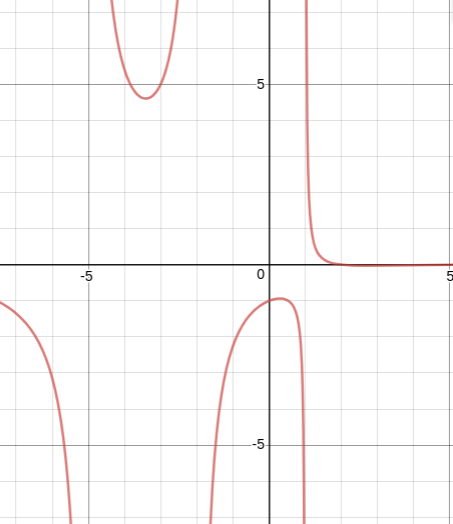
\includegraphics[width=0.5\textwidth]{../Figures/identifyGraphOfRationalFunctionCopyC.png}
\end{center}
\begin{enumerate}[label=\Alph*.]
\item \( f(x)=\frac{x^{3} + x^{2} -14 x -24}{x^{3} +15 x^{2} +68 x + 84} \)
\item \( f(x)=\frac{x^{3} -3 x^{2} -10 x + 24}{x^{3} +15 x^{2} +68 x + 84} \)
\item \( f(x)=\frac{x^{3} -1 x^{2} -14 x + 24}{x^{3} -15 x^{2} +68 x -84} \)
\item \( f(x)=\frac{x^{3} -1 x^{2} -14 x + 24}{x^{3} -15 x^{2} +68 x -84} \)
\item \( \text{None of the above are possible equations for the graph.} \)

\end{enumerate} }
\litem{
Determine the vertical asymptotes and holes in the rational function below.\[ f(x) = \frac{16x^{3} -32 x^{2} -113 x -60}{12x^{2} -5 x -25} \]\begin{enumerate}[label=\Alph*.]
\item \( \text{Vertical Asymptotes of } x = 1.667 \text{ and } x = -0.75 \text{ with a hole at } x = -1.25 \)
\item \( \text{Vertical Asymptote of } x = 1.667 \text{ and hole at } x = -1.25 \)
\item \( \text{Holes at } x = 1.667 \text{ and } x = -1.25 \text{ with no vertical asymptotes.} \)
\item \( \text{Vertical Asymptotes of } x = 1.667 \text{ and } x = -1.25 \text{ with no holes.} \)
\item \( \text{Vertical Asymptote of } x = 1.333 \text{ and hole at } x = -1.25 \)

\end{enumerate} }
\litem{
Determine the vertical asymptotes and holes in the rational function below.\[ f(x) = \frac{6x^{3} +7 x^{2} -35 x -50}{6x^{2} -7 x -20} \]\begin{enumerate}[label=\Alph*.]
\item \( \text{Holes at } x = -1.333 \text{ and } x = 2.5 \text{ with no vertical asymptotes.} \)
\item \( \text{Vertical Asymptote of } x = 1.0 \text{ and hole at } x = 2.5 \)
\item \( \text{Vertical Asymptotes of } x = -1.333 \text{ and } x = 2.5 \text{ with no holes.} \)
\item \( \text{Vertical Asymptotes of } x = -1.333 \text{ and } x = -1.667 \text{ with a hole at } x = 2.5 \)
\item \( \text{Vertical Asymptote of } x = -1.333 \text{ and hole at } x = 2.5 \)

\end{enumerate} }
\end{enumerate}

\end{document}